%% ----------------------------------------------------------------
%% Thesis.tex
%% ---------------------------------------------------------------- 
%% Final copy must be double sided printing.
\documentclass[twoside]{ecsthesis}      % Use the Thesis Style
\graphicspath{{../Figures/}}   % Location of your graphics files
\usepackage{natbib}            % Use Natbib style for the refs.
%% \removecolourlinks    % Uncomment this command to remove colour from any links
%% ----------------------------------------------------------------
%% Definitions.tex
%% ---------------------------------------------------------------- 


\newcommand{\BibTeX}{{\rm B\kern-.05em{\sc i\kern-.025em b}\kern-.08em T\kern-.1667em\lower.7ex\hbox{E}\kern-.125emX}}

%% People
\newcounter{address}
\setcounter{address}{1}
\renewcommand{\theaddress}{\textsuperscript{\fnsymbol{address}}}
\newcommand{\address}[1]{\refstepcounter{address}\theaddress#1\\}
\newcommand{\Name}[3]{\texorpdfstring{\href{mailto:#3}{#2}#1}{#2}\xspace}
\newcommand{\SteveRGunn}[1]{\Name{#1}{Steve R. Gunn}{S.R.Gunn@ecs.soton.ac.uk}}

%% Dingbats
\newcommand{\tick}{\ding{51}}
\newcommand{\cross}{\ding{55}}

%% Calculus
\newcommand{\pd}[2]{\ensuremath{\frac{\partial #1}{\partial #2}}\xspace}
\newcommand{\fd}[2]{\ensuremath{\frac{d #1}{d #2}}\xspace}
\newcommand{\dint}{\ensuremath{\int\!\!\!\int}\xspace}
\newcommand{\tint}{\ensuremath{\int\!\!\!\int\!\!\!\int}\xspace}

%% Math Sets
\newcommand{\Q}[1]{\ensuremath{\mathbb{#1}}\xspace}
\newcommand{\R}{\Q{R}}

%% Matrix, Vector
\newcommand{\V}[1]{\ensuremath{\boldsymbol{#1}}\xspace}
\newcommand{\M}[1]{\ensuremath{\boldsymbol{#1}}\xspace}
\newcommand{\0}{\V{0}}
\newcommand{\1}{\V{1}}
\newcommand{\I}{\M{I}}

%% Math Functions
\newcommand{\F}[1]{\ensuremath{\mathrm{#1}}\xspace}
\newcommand{\sgn}{\F{sgn}}
\newcommand{\tr}{\F{trace}}
\newcommand{\diag}{\F{diag}}

%% Math Names
\newcommand{\N}[1]{\ensuremath{\mathit{#1}}\xspace}

%% Data
\newcommand{\mc}[1]{\ensuremath{\mathcal{#1}}\xspace}
\newcommand{\Hyp}{\mc{H}}
\newcommand{\D}{\mc{D}}

%% Kernel
\newcommand{\K}{\M{K}}
\newcommand{\eins}{\texorpdfstring{\ensuremath{\epsilon}}{\textepsilon}-insensitive\xspace}
\newcommand{\e}{\ensuremath{\epsilon}\xspace}
\newcommand{\Bxi}{\ensuremath{\boldsymbol{\xi}}\xspace}
\newcommand{\Kanova}{\ensuremath{\mathit{K_{ANOVA}}}\xspace}
\newcommand{\Kspline}{\ensuremath{\mathit{K_{spline}}}\xspace}

%% Bayesian
\newcommand{\MP}{\ensuremath{\mathit{{\scriptscriptstyle \hspace{-1.5pt}M\hspace{-1.5pt}P}}}\xspace}
\newcommand{\ML}{\ensuremath{\mathit{{\scriptscriptstyle \hspace{-1.5pt}M\hspace{-1.5pt}L}}}\xspace}
\newcommand{\Qw}{\ensuremath{Q_{\w}(\w)}\xspace}
\newcommand{\Qa}{\ensuremath{Q_{\Ba}(\Ba)}\xspace}
\newcommand{\Qb}{\ensuremath{Q_{\beta}(\beta)}\xspace}
\newcommand{\wMPab}{\ensuremath{\w_{\MP|\bar {\Ba},\bar \beta}}\xspace}
\newcommand{\wMP}{\ensuremath{\w_{\MP}}\xspace}
\newcommand{\yMP}{\ensuremath{y_{\MP}}\xspace}
\newcommand{\BaMP}{\ensuremath{\Ba_{\hspace{1pt}\MP}}\xspace}
\newcommand{\aMP}{\ensuremath{\alpha_{\hspace{1pt}\MP}}\xspace}
\newcommand{\bMP}{\ensuremath{\beta_{\hspace{1pt}\MP}}\xspace}
\newcommand{\Sab}{\ensuremath{\M{\Sigma}_{\bar \Ba,\bar \beta}}\xspace}
\newcommand{\Ba}{\ensuremath{\boldsymbol{\alpha}}\xspace}
\newcommand{\Bb}{\ensuremath{\boldsymbol{\beta}}\xspace}
\newcommand{\Bm}{\ensuremath{\boldsymbol{\mu}}\xspace}
\newcommand{\BL}{\ensuremath{\boldsymbol{\Lambda}}\xspace}
\newcommand{\BPhi}{\ensuremath{\boldsymbol{\Phi}}\xspace}
\newcommand{\SMP}{\ensuremath{\M{\Sigma}_{\MP}}\xspace}

\newcommand{\Pa}{\ensuremath{P(\alpha|\mathcal{H})}\xspace}
\newcommand{\Pb}{\ensuremath{P(\beta|\mathcal{H})}\xspace}
\newcommand{\Pab}{\ensuremath{P(\alpha,\beta|\mathcal{H})}\xspace}
\newcommand{\Pw}{\ensuremath{P(\w|\mathcal{H})}\xspace}
\newcommand{\PD}{\ensuremath{P(\D|\mathcal{H})}\xspace}
\newcommand{\PwIa}{\ensuremath{P(\w|\alpha,\mathcal{H})}\xspace}
\newcommand{\PDIwb}{\ensuremath{P(\D|\w,\beta,\mathcal{H})}\xspace}
\newcommand{\PDwab}{\ensuremath{P(\D,\w,\alpha,\beta|\mathcal{H})}\xspace}
\newcommand{\PDIw}{\ensuremath{P(\D|\w,\mathcal{H})}\xspace}
\newcommand{\PwID}{\ensuremath{P(\w|\D,\mathcal{H})}\xspace}
\newcommand{\PwabID}{\ensuremath{P(\w,\alpha,\beta|\D,\mathcal{H})}\xspace}

\newcommand{\PanH}{\ensuremath{P(\alpha)}\xspace}
\newcommand{\PbnH}{\ensuremath{P(\beta)}\xspace}
\newcommand{\PabnH}{\ensuremath{P(\alpha,\beta)}\xspace}
\newcommand{\PwnH}{\ensuremath{P(\w)}\xspace}
\newcommand{\PDnH}{\ensuremath{P(\D)}\xspace}
\newcommand{\PwIanH}{\ensuremath{P(\w|\alpha)}\xspace}
\newcommand{\PDIwbnH}{\ensuremath{P(\D|\w,\beta)}\xspace}
\newcommand{\PDwabnH}{\ensuremath{P(\D,\w,\Ba,\beta)}\xspace}
\newcommand{\PDIwnH}{\ensuremath{P(\D|\w)}\xspace}
\newcommand{\PwIDnH}{\ensuremath{P(\w|\D)}\xspace}
\newcommand{\PwabIDnH}{\ensuremath{P(\w,\alpha,\beta|\D)}\xspace}

\newcommand{\PDwBab}{\ensuremath{P(\D,\w,\Ba,\beta|\mathcal{H})}\xspace}
\newcommand{\PwIBa}{\ensuremath{P(\w|\Ba,\mathcal{H})}\xspace}
\newcommand{\PBab}{\ensuremath{P(\Ba,\beta|\mathcal{H})}\xspace}
\newcommand{\PwBabID}{\ensuremath{P(\w,\Ba,\beta|\D,\mathcal{H})}\xspace}

\newcommand{\PBanH}{\ensuremath{P(\Ba)}\xspace}
\newcommand{\PwIBanH}{\ensuremath{P(\w|\Ba)}\xspace}

%% Snakes
\newcommand{\Esnake}{\ensuremath{\mathit{E_{snake}}}\xspace}
\newcommand{\Eimage}{\ensuremath{\mathit{E_{image}}}\xspace}
\newcommand{\Econt}{\ensuremath{\mathit{E_{cont}}}\xspace}
\newcommand{\Ecurv}{\ensuremath{\mathit{E_{curv}}}\xspace}
\newcommand{\Eint}{\ensuremath{\mathit{E_{int}}}\xspace}
\newcommand{\Eext}{\ensuremath{\mathit{E_{ext}}}\xspace}
\newcommand{\Eterm}{\ensuremath{\mathit{E_{term}}}\xspace}
\newcommand{\Eline}{\ensuremath{\mathit{E_{line}}}\xspace}
\newcommand{\Eedge}{\ensuremath{\mathit{E_{edge}}}\xspace}
\newcommand{\Econ}{\ensuremath{\mathit{E_{con}}}\xspace}
\newcommand{\Eangle}{\ensuremath{\mathit{E_{angle}}}\xspace}
\newcommand{\Elshape}{\ensuremath{\mathit{E_{lshape}}}\xspace}
\newcommand{\Eedgedir}{\ensuremath{\mathit{E_{edgedir}}}\xspace}
\newcommand{\Emodel}{\ensuremath{\mathit{E_{model}}}\xspace}
\newcommand{\wte}{\ensuremath{\mathit{w_{term}}}\xspace}
\newcommand{\wli}{\ensuremath{\mathit{w_{line}}}\xspace}
\newcommand{\wed}{\ensuremath{\mathit{w_{edge}}}\xspace}
\newcommand{\wco}{\ensuremath{\mathit{w_{con}}}\xspace}

%% Environments
\newcounter{alg}
\newenvironment{algorithm}[1]
{
    \stepcounter{alg}
    \begin{table}[htb]
    \centering
    \begin{tabular}[t]{ll}
    \hline&\\
    \multicolumn{2}{l}{\bf Algorithm \arabic{alg}: #1}\\&\\
} {
    &\\
    \hline
    \end{tabular}
    \end{table}
}
            % Include your abbreviations
%% ----------------------------------------------------------------
\begin{document}
\frontmatter
\title      {Using Linked Data in Purposive Social Networks}
\authors    {\texorpdfstring
             {\href{mailto:ps1w07@ecs.soton.ac.uk}{Priyanka Singh}}
             {Priyanka Singh}
            }
\department  {Electronics and Computer Science}
\group       {Web and Internet Science}
\addresses  {\groupname\\\deptname\\\univname}
\date       {\today}
\subject    {}
\keywords   {}
\maketitle
\begin{abstract}
This work is all about \dots
\end{abstract}
\tableofcontents
\listoffigures
\listoftables

%% -----------------------
%% lstpatch.sty
%% -----------------------
%% lstpatch cannot be distributed with these files. I believe it is only needed if the
%% \lstlistoflistings is used. So this has been turned off by default. Re-add if required:
%% \usepackage{lstpatch}
%% \lstlistoflistings
%% You will need to download lstpatch, possibly from:
%% http://web.mit.edu/texsrc/source/latex/listings/lstpatch.sty
%% -----------------------


%% -----------------------
%% Authorship declaration
%% -----------------------
%% Either include citations like below (as many as required spaced with commas or 'and').
\authorshipdeclaration{\citep{Gunn:2001:pdflatex}, \citep{Lovell:2011:updated} and \citep{Gunn:2011:updated2}}
%% Or state no citations like below
%% \authorshipdeclaration{}
%% -----------------------

\acknowledgements{Thanks to no one.}
\listofsymbols{ll}{$w$ & The weight vector}
\mainmatter
%% ----------------------------------------------------------------
%% ----------------------------------------------------------------
%% Introduction.tex
%% ---------------------------------------------------------------- 


\chapter{Introduction} \label{Chapter:Introduction}
Hello

\section{Overview}
\section{Research Challenge}
\section{Research Contribution}
\section{Structure of Thesis}
%% ----------------------------------------------------------------
%% Background.tex
%% ---------------------------------------------------------------- 


\chapter{Background} \label{Chapter:Background}
Hello

\section{Emergence of Social Web}
\subsection{Web 2.0 and Social Networks}
\subsection{Content-specific Social Networking Services}

\section{Collective Intelligence and Crowdsourcing}

\subsection{Crowdsourcing Services}
\subsubsection{Wiki}
\subsubsection{Forums and Messaging Boards}
\subsubsection{Q\&A Services}
\subsection{Human Computation}
\subsection{User Recommendation System}

\section{Semantic Web and Linked Data}
\subsection{Social Semantic Technology}
\subsubsection{FOAF}
\subsubsection{SIOC}
\subsubsection{OPO}
\subsection{Linked Data Technology}
\subsubsection{Linking the Datasets}
\subsection{Open Linked Data and Graph}

\section{Semantic Search}
\subsection{Keyword Disambiguation}
\subsection{Concept Mapping}
\subsection{SPARQL Queries}
%% ----------------------------------------------------------------
%% PSN.tex
%% ---------------------------------------------------------------- 


\chapter{Purposive Social Network} \label{Chapter:Purposive Social Network}
Hello

\section{What is Purposive Social Network}
\subsection{Information Based Community}
\subsection{Interest Based Community}
\subsection{Expert Based Community}
\subsection{Location Based Community}

\section{Characteristics of Purposive Social Network}
\subsection{Community Size}
\subsection{Focused Interest}
\subsection{Direct Communication}
\subsection{Active Participation}
\subsection{Short Lifespan}
\subsection{Strong Incentive}

\section{Benefits of Purposive Social Network}
\subsection{Information Exchange and Self-interest}
\subsection{Symbiotic Relation and Social Exchange}
\subsection{Social Recognition and Personal Satisfaction}
\subsection{Recommendation System}
\subsection{Expert Finder}

\section{Crowdsourcing in Purposive Social Network}
\subsection{Recruiting and Retaining Users}
\subsection{Incentive Model}
\subsection{Quality Control}
\subsection{Search and Discovery of Quality Content}

\section{Use of Semantic Web and Linked Data in Purposive Social Network}
\subsection{Structured Data}
\subsection{Linking People to People and People to Data}
\subsection{Multidimensional Network and Graph}
\subsection{Integrated Knowledgebase}
\subsection{Smart Query and Search}
\subsection{Social Network Analysis}
%% ----------------------------------------------------------------
%% System.tex
%% ---------------------------------------------------------------- 


\chapter{System Design and Methodology} \label{Chapter:System Design and Methodology}
Hello

\section{Data Mining}
\subsection{StackOverflow Data Mining}
\subsection{Reddit Data Mining}

\section{Data Structuring}

The data extracted from StackOverflow website is in the form of simple text, some of the posts contain HTML codes but they are snippets of code and are represented as text in the database. The users categorize the posts by using tags and it gives information about the topic and the programming language the question is being asked. The answers do not have special tags but the tags of the questions are applied to the answers as well.


\subsection{Data Cleaning}
\subsection{Converting into N-Triples}

All the user data, post data, votes and badges are transformed in RDF data by applying simple RDF schema and ontologies.

The website only shows basic user profile information due to the privacy reasons and FOAF ontology is used to describe the data. An example of the simple user profile information is as follows:

\begin{verbatim}
<foaf:Person>
    <foaf:name> Geoff Dalgas </foaf:name>
    <foaf:mbox_sha1sum> b437f461b3fd27387c5d8ab47a293d35 </foaf:mbox_sha1sum>
    <foaf:based_near> Corvallis, OR </foaf:based_near>
    <foaf:age> 35 </foaf:age>
    <foaf:OnlineAccount> http://stackoverflow.com/users/2/geoff-dalgas 
    </foaf:OnlineAccount
</foaf:Person>
 \end{verbatim}
 
 Similarly, the posts created by users, the questions and answers are described using SIOC ontology. The content is described and linked with the user RDF using the similar URIs.
 
\begin{verbatim}
<sioc:Post rdf:about=" http://stackoverflow.com/questions/89228/calling-an-external
-command-in-python">
    <dcterms:title>Calling an external command in Python</dcterms:title>
    <dcterms:created> 2008-09-18T21:42:52.667 </dcterms:created>
    <sioc:has_container rdf:resource=" http://stackoverflow.com/questions/tagged
    /python"/>
    <sioc:has_creator>
       <sioc:UserAccount rdf:about=" http://stackoverflow.com/users/170339/bludger " 
       rdfs:label="bludger"> </sioc:UserAccount>
     </sioc:has_creator>
     <sioc:content>How can I call an external command in Python</sioc:content>
     <sioc:topic rdfs:label="python" rdf:resource=" http://stackoverflow.com
       /questions/tagged/python"/>
     <sioc:topic rdfs:label="command" rdf:resource=" http://stackoverflow.com
       /questions/tagged/command"/>
     <sioc:has_reply>
        <sioc:Post rdf:about=" http://stackoverflow.com/a/89243/1313327">
            <sioc:content>Look at the subprocess module in the stdlib: from subprocess 
             import call call(["ls", "-l"]) The advantage of subprocess vs system is that 
             it is more flexible (you can get the stdout, stderr, the "real" status code, 
             better error handling, etc...). I think os.system is deprecated, too, or will
             be: http://docs.python.org/library/subprocess.html#replacing-older-functions
             -with-the-subprocess-module For quick/dirty/one time scripts, os.system
             is enough, though.</sioc:content>
             <dcterms:created>2008-09-18T23:42:52.667</dcterms:created>
             <sioc:has_creator>
                <sioc:UserAccount rdf:about=" http://stackoverflow.com/users/11465
                 /david-cournapeau" rdfs:label=" david-cournapeau "> </sioc:UserAccount>
              </sioc:has_creator>
           </sioc:Post>
      </sioc:has_reply>
</sioc:Post>
\end{verbatim}

\subsection{Linking the Data}

\section{Keyword Disambiguation}
\subsection{OpenCalais Service}
\subsection{DBpedia Spotlight Service}

\section{Concept Mapping}
\subsection{Keyword Matrix}
\subsection{Document Term Matrix}

\section{Search and Query}
\subsection{Database Design}
\subsection{Searching Answers of Unanswered Questions}
\subsection{Expert Finder}
%% ----------------------------------------------------------------
%% Analysis.tex
%% ---------------------------------------------------------------- 


\chapter{Analysis of Purposive Social Network} \label{Chapter: Analysis of Purposive Social Network}

A purposive social network is a broad and general concept that can be applied to many different social networks. At its core, it is a network with a specific goal and purpose where people come together to solve a particular problem.

For this research StackOverflow website is analyzed where programmers and developers ask questions and experts in the field answer them and solve the problem. In this analysis, the user asking and answering questions, voting the responses and commenting are the main entities of the social network. Their network ties are measured by their communication and interaction between them. The amount of their contribution is measured by the crowdsourcing where people give up votes or down votes to their posts and the badges they receive for their contribution.

\section{Network Linkage and Social Ties}

StackOverflow is not a typical social networking website per se as users cannot create an explicit friendship or follow other people�s work, they cannot send private messages or form groups.

The social ties are form implicit by user interaction with each other through asking questions and answering them, voting on the posts and commenting on them. The communication network is studied to see the social ties of the individuals \cite{monge2003theories}.

\begin{table}[!htb]
  \centering
  \begin{tabular}{cc}
  \toprule
  \textbf{Post Type} & \textbf{Number}\\
  \midrule
   Questions & 3279233\\   \midrule
   Answers & 6578079\\   \midrule
   Registered Users & 1225580\\   \midrule
   Tags & 30408 \\   \midrule
   Unanswered Questions & 780535\\   \midrule
   Badges & 3454994\\   \midrule
   Votes & 26184363\\   \midrule
   Comments & 12526162\\ 
  \bottomrule
  \end{tabular}
  \caption{StackOverflow at glance as of June 2012}
  \label{Table:tabex}
\end{table}

As of June 2012, there are over one million registered users in StackOverflow and more than 3.2 millions questions asked by users. The questions are categorized using tags and individual users can subscribe to tags to receive daily email of all the question asked in the tag. There are more than 30 thousand tags associated with various questions and answers. Users have casted more than 26 million votes to mark the good questions and answers.

\begin{figure}[!htb]
  \centering
  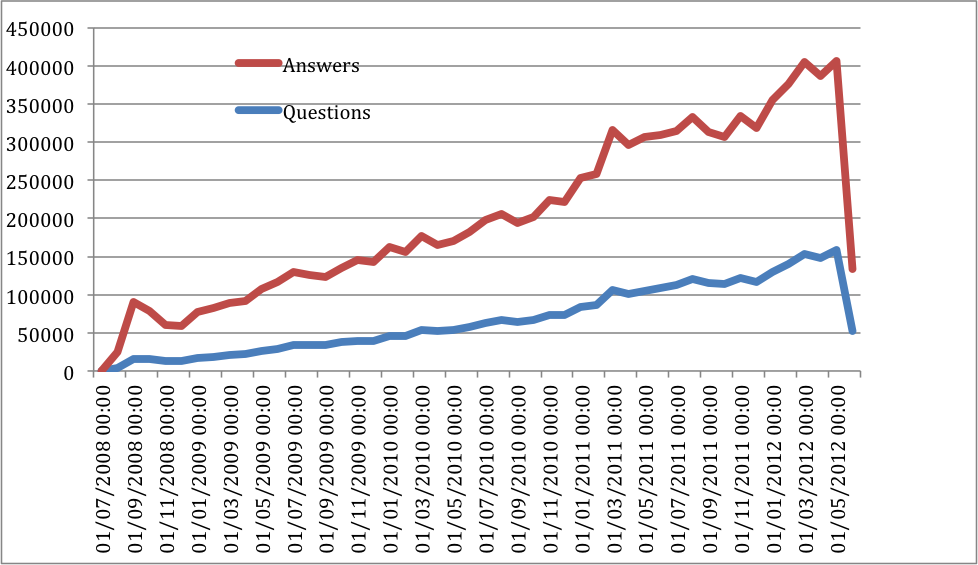
\includegraphics[width=15cm]{qa.png}
  \caption{Questions and answers posted per month on StackOverflow}
  \label{Figure:figex4a}
\end{figure}

The \fref{Figure:figex4a} shows the number of questions asked and answered by users each month. In the year 2012, each questions have on average 1.645 number of answers.

This community is made of programmers and their motivation is to solve the problem they had encountered and to provide answers to gain reputations. Thousands of questions and answers are posted everyday. The analysis of posts shows that the programmers prefer to ask the questions and answers on weekdays.

\begin{figure}[!htb]
  \centering
  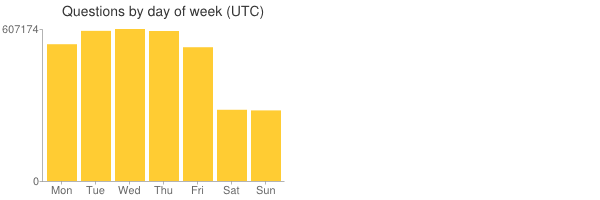
\includegraphics[width=15cm]{chart1.png}
  \caption{Questions posted by the day of week}
  \label{Figure:figex4b}
\end{figure}

Despite high user feedback and participation, 23.79\% of questions are not answered or the answers do not receive any up votes. On average a question receives 2.006 answers and .12\% of questions receives more than 15 answers.

\begin{figure}[!htb]
  \centering
  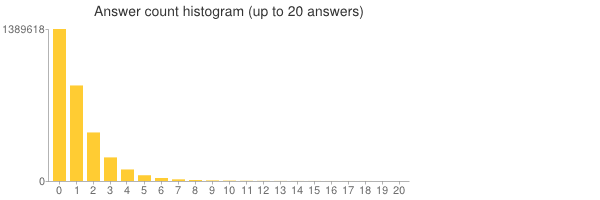
\includegraphics[width=15cm]{chart2.png}
  \caption{Answer count to the questions}
  \label{Figure:figex4c}
\end{figure}

The questions are answers are provided with tags to categorize and arrange for easy search and discovery. The entire website is categorized using the tags and the list of most popular tags are shown in the table. The figure shows the weekly use of the popular tags. The number of questions asked for each tags also provides an insight on the popular language used by developers at the time.

\begin{table}[!htb]
  \centering
  \begin{tabular}{cc}
  \toprule
  \textbf{Tags} & \textbf{Number of instance}\\  \midrule
   C\# & 370074 \\ \midrule
   JAVA &  315488 \\ \midrule
   PHP & 293755 \\ \midrule
   JavaScript & 278592 \\ \midrule
   Android & 244791 \\
  \bottomrule
  \end{tabular}
  \caption{Five most popular tags and its instances}
  \label{Table:tabex2}
\end{table}

\begin{figure}[!htb]
  \centering
  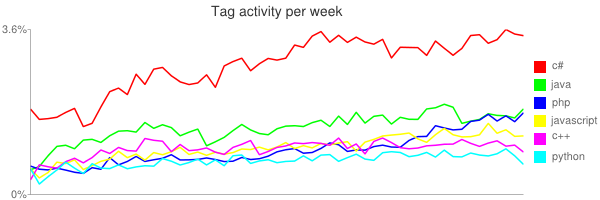
\includegraphics[width=15cm]{chart3.png}
  \caption{Tag trends per week of most popular tags}
  \label{Figure:figex4d}
\end{figure}

The analysis of questions shows that each question has between one to five tags associated with it. Most questions (70.30\%) have 2 to 4 tags associated with it. The relationship between the tags shows the overlapping of networks and how it is tied with one another.

\cite{Eberhardt2012} provided an interactive graph in his website to show the relationships between the most popular tags and how closely they are related to each other. In the following graph each segment size is directly proportional to the number of instance it is used and the connection between the tags indicate the times they have been used together in a question. The thickness of the connection shows the strength of the relations. The segment is colour coded by the frequency of connections, red segments are strongly connected and blue segments are weakly connected.

\begin{figure}[!htb]
  \centering
  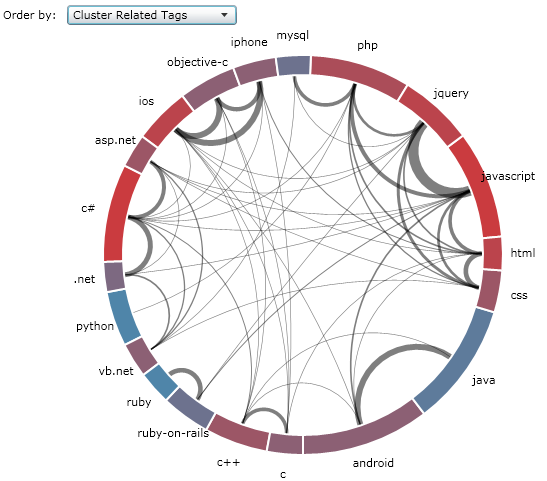
\includegraphics[width=11cm]{graph1.png}
  \caption{Related tags clustered together}
  \label{Figure:figex4e}
\end{figure}

\begin{figure}[!htb]
  \centering
  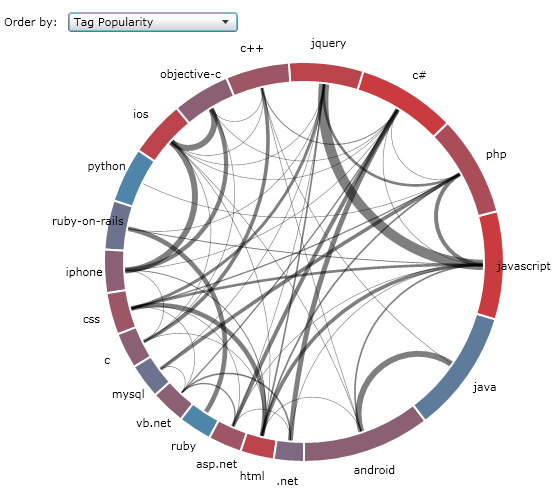
\includegraphics[width=11cm]{graph2.png}
  \caption{Popular tags clustered together}
  \label{Figure:figex4f}
\end{figure}

The clustering of the tags shows the relationship between the tags and technologies. The two popular tags JAVA and Android are closely related to each other but are scarcely joined with other tags. The strongest relationship is between jQuery and JavaScript because the overlapping framework of the two programming languages. C, C++ and C\# are also a closely related groups as well as iOS, Objective-C and iPhone. However, sometimes Objective-C is also tagged with C, C++ and C\#, if by mistake or deliberately can be argued.
There is a large cluster of connected web development languages, CSS, HTML, JavaScript and jQuery, indicating the close knit use of these technologies in development of website and web applications. The interesting thing is the relationship between the scripting langue PHP and Python, they are popular tags but are sparsely connected with other tags and are weakly linked with database related tags.

\section{Role of Individual Actors}

Users who contribute to the website are the main actors of this purposive social network. There are more than 1.2 million registered users in StackOverflow and they ask the questions, answer it, vote it and moderate the community. The users are not directly linked to each other to create relationships; in this network the relationship is formed by their interaction and their contribution. The user behaviour, their motivation to use the website and incentive to contribute is described below.

Despite the high content generation by the users, 56.02\% do not interact or contribute to the website, they have 1 reputation point that they receive while joining the website.

\begin{figure}[!htb]
  \centering
  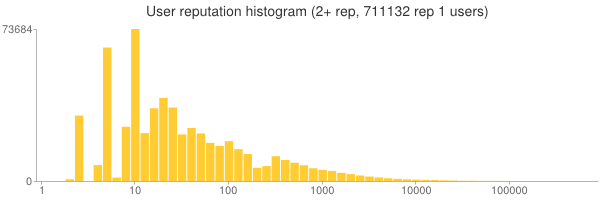
\includegraphics[width=15cm]{chart4.png}
  \caption{User reputation histogram}
  \label{Figure:figex4g}
\end{figure}

\begin{table}[!htb]
  \centering
  \begin{tabular}{cc}
  \toprule
  \textbf{Reputation} & \textbf{Number of users}\\  \midrule
  1 & 669554\\ \midrule
  2-10 & 126235\\ \midrule
  11-100 & 295389\\ \midrule
  101-1000 & 3161130\\  \midrule
  1001-10000 & 170993\\ \midrule
  10001-20000 & 1437\\ \midrule
  20001-100000 & 895\\ \midrule
  100001-200000 & 49\\ \midrule
  less than 200000 & 11\\
  \bottomrule
  \end{tabular}
  \caption{Number of users with reputations}
  \label{Table:tabex3}
\end{table}

As \tref{Table:tabex3} shows, there are 669554 users with 1 reputation point and one user with 452951 reputation points. The distribution of the users reputation shows that more than half of the users are lurkers and the elite users with the most reputation points are the editors and moderators of the community and are considered the expert in their field.

The reputation of the user has a direct correlation with the trust in the community. StackOverflow has designed an excellent reward program to motivate and incentivize the users to contribute and gain more reputations and badges.

Currently, there are 77 different types of badges given to the user based on their contribution. There are badges given to the user who asks questions with 1 reputation point (Student), to the user who edits the answers to make posts better (Editor) and to even an active user for a year (Yearling). This type of virtual acknowledgement of efforts encourage the user to participate and contribute to the website.

The other method that encourages the users to participate is the promptness of the response. The asker prefers to receive information sooner rather than later, and will stop the process when satisfied with the cumulative value of the posted information. The analysis of the posts shows that half of the questions get an answer within an hour of the posting and within a day the questions receives an accepted answer. When the answers are delayed, the questioners look for alternative websites to get a response.

\begin{figure}[!htb]
  \centering
  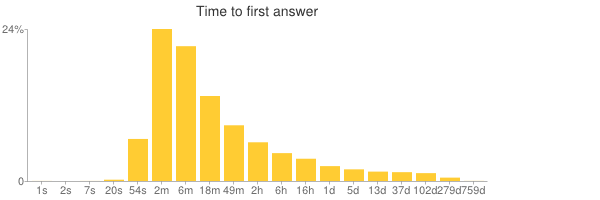
\includegraphics[width=15cm]{chart5.png}
  \caption{Time to receive the first answer}
  \label{Figure:figex4h}
\end{figure}

\begin{figure}[!htb]
  \centering
  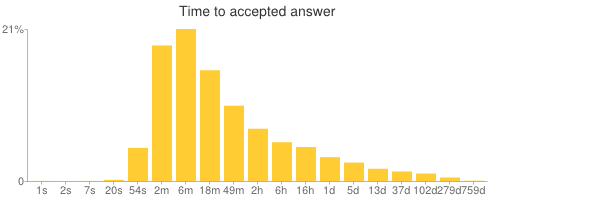
\includegraphics[width=15cm]{chart6.png}
  \caption{Time to get the accepted answer}
  \label{Figure:figex4i}
\end{figure}

\section{Incentive Design and Quality Control}

The StackOverflow website uses a game theoretic model to encourage user participation and activity. Participation is encouraged through an elaborate point system and users also receive badges for participation. Also, the top contributor and user with highest reputation are featured on the question page, giving the user more visibility and acknowledgement of the user�s expertise. This encourages participants to accumulate more points and contribute to get recognition.

When an answer is votes up, the user gains 10 reputations and 5 points when the question is voted up. When an answer is accepted the user receives 15 points and there is also negative point system, a user looses 2 reputation point when a question or an answer is voted down. This keeps the spamming in check and repeated questions and answers are avoided.

The system also encourages users to participate as the higher reputation points gain more privileges. When a user has 15 reputation points, only then they can up vote and 50 points allows users to comment. To stop harassment and spam, user requires 125 reputation points to vote down and it costs the user 1 reputation point. The incentive model is thorough and higher reputation points open more gates for users to interact and contribute and be acknowledged as the expert in their field.

The community thrives because of the high quality of content and it is possible by the user�s action and moderation. Users vote up the good questions and answers and vote down the bad quality content or repeated posts. There is more than 6 million votes casted in the website and the user with enough reputations are allowed to cast 40 votes per day.

\begin{figure}[!htb]
  \centering
  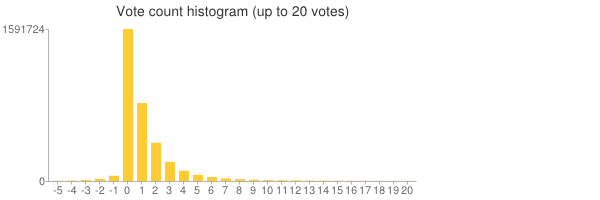
\includegraphics[width=15cm]{chart7.png}
  \caption{Vote count histogram}
  \label{Figure:figex4j}
\end{figure}

\begin{table}[!htb]
  \centering
  \begin{tabular}{cc}
  \toprule
  \textbf{Vote} & \textbf{Vote Count}\\  \midrule
  less than 20 & 25\\  \midrule
  0 & 504754\\  \midrule
  1-10 & 7802690\\  \midrule
  11-100 & 718650\\  \midrule
  101-1000 & 6460\\  \midrule
  1000-5000 &11\\
  \bottomrule
  \end{tabular}
  \caption{Questions� votes count}
  \label{Table:tabex4}
\end{table}

The analysis of the questions and votes shows that every question receives 3.06 votes on average. One question received negative 115 votes and the highest vote received to a question is 2499. Similar analysis of answers and their votes shows that, on average an answer receives 0.99 votes and the lowest vote to an answer is negative 57 and the highest vote is 4432.

\section{Using Semantic Web Technologies}

The data extracted from StackOverflow website is in the form of simple text, some of the posts contain HTML codes but they are snippets of code and are represented as text in the database. The users categorize the posts by using tags and it gives information about the topic and the programming language the question is being asked. The answers do not have special tags but the tags of the questions are applied to the answers as well.

\subsection{Using RDF and Linked Data}

All the user data, post data, votes and badges are transformed in RDF data by applying simple RDF schema and ontologies.

The website only shows basic user profile information due to the privacy reasons and FOAF ontology is used to describe the data. An example of the simple user profile information is as follows:

\begin{verbatim}
<foaf:Person>
    <foaf:name> Geoff Dalgas </foaf:name>
    <foaf:mbox_sha1sum> b437f461b3fd27387c5d8ab47a293d35 </foaf:mbox_sha1sum>
    <foaf:based_near> Corvallis, OR </foaf:based_near>
    <foaf:age> 35 </foaf:age>
    <foaf:OnlineAccount> http://stackoverflow.com/users/2/geoff-dalgas 
    </foaf:OnlineAccount
</foaf:Person>
 \end{verbatim}
 
 Similarly, the posts created by users, the questions and answers are described using SIOC ontology. The content is described and linked with the user RDF using the similar URIs.
 
\begin{verbatim}
<sioc:Post rdf:about=" http://stackoverflow.com/questions/89228/calling-an-external
-command-in-python">
    <dcterms:title>Calling an external command in Python</dcterms:title>
    <dcterms:created> 2008-09-18T21:42:52.667 </dcterms:created>
    <sioc:has_container rdf:resource=" http://stackoverflow.com/questions/tagged
    /python"/>
    <sioc:has_creator>
       <sioc:UserAccount rdf:about=" http://stackoverflow.com/users/170339/bludger " 
       rdfs:label="bludger"> </sioc:UserAccount>
     </sioc:has_creator>
     <sioc:content>How can I call an external command in Python</sioc:content>
     <sioc:topic rdfs:label="python" rdf:resource=" http://stackoverflow.com
       /questions/tagged/python"/>
     <sioc:topic rdfs:label="command" rdf:resource=" http://stackoverflow.com
       /questions/tagged/command"/>
     <sioc:has_reply>
        <sioc:Post rdf:about=" http://stackoverflow.com/a/89243/1313327">
            <sioc:content>Look at the subprocess module in the stdlib: from subprocess 
             import call call(["ls", "-l"]) The advantage of subprocess vs system is that 
             it is more flexible (you can get the stdout, stderr, the "real" status code, 
             better error handling, etc...). I think os.system is deprecated, too, or will
             be: http://docs.python.org/library/subprocess.html#replacing-older-functions
             -with-the-subprocess-module For quick/dirty/one time scripts, os.system
             is enough, though.</sioc:content>
             <dcterms:created>2008-09-18T23:42:52.667</dcterms:created>
             <sioc:has_creator>
                <sioc:UserAccount rdf:about=" http://stackoverflow.com/users/11465
                 /david-cournapeau" rdfs:label=" david-cournapeau "> </sioc:UserAccount>
              </sioc:has_creator>
           </sioc:Post>
      </sioc:has_reply>
</sioc:Post>
\end{verbatim}

\subsection{Topic Disambiguation}

The StackOverflow dataset is sparsely annotated by user-generated tags and it is not linked with any other datasets. When user creates a question, they add tags to it to categorize into different topics but the answers have the tags from the questions. Also, all the main topics inside the text of question or answer is not clearly stated. The topics are ambiguous and not linked to any vocabulary or properly annotated.

A sample of the question, answer and tag data is annotated with the links from Wikipedia datasets and Drupal datasets to resolve the name and topic disambiguation. These services do the name entity recognition and match the entities with the appropriate topics and categories. The service does not convert the text into Linked Data or RDF, the returned data is further transformed into RDF and linked with the DBpedia dataset.

Wikipedia Miner service is used to annotate a small sample of posts, the service returns the text with annotated topics embedded into the text. The service accepts simple text or HTML and one can specify the density of links to be added and the level of accuracy required from the service. Below is an example annotated text of a question and answer posted.

\begin{figure}[!htb]
  \centering
  \subfigure[Annotating a text question]{
    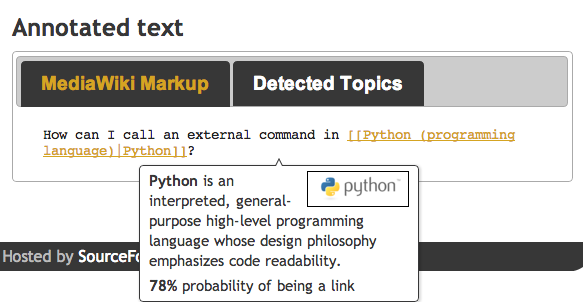
\includegraphics[width=14cm]{q.png}
    \label{Figure:figsubex11:left}
  }
  \subfigure[Annotating a text answer]{
    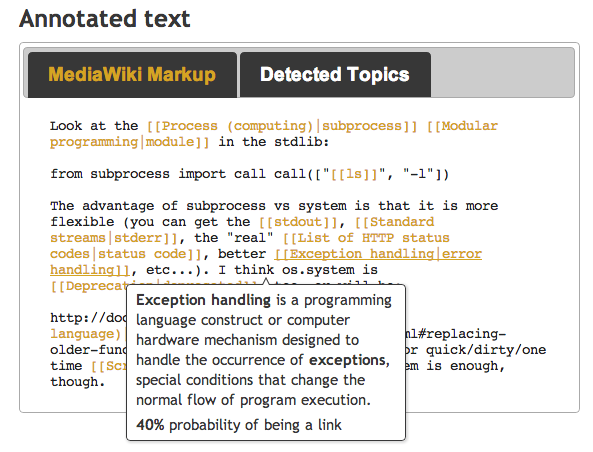
\includegraphics[width=14cm]{ans.png}
    \label{Figure:figsubex11:right}
  }
  \caption{Wikipedia Miner web service annotating a text question and an answer}
  \label{Figure:figsubex11}
\end{figure}

The Wikipedia miner service uses a word sense disambiguation based machine learning algorithm and where it detects key terms in a text excerpt and disambiguating then against Wikipedia article. It provides a JAVA API to access the Wikipedia database, including all the categories and it can be searched, browsed and iterated over \cite{milne2012open}.

OpenCalais is another web service used to annotate the StackOverflow posts with the Drupal dataset. This tool creates a semantic rich metadata for the content using the natural language processing, machine learning and name disambiguation algorithm. It provides many services; it provides tag integration with different taxonomy and vocabulary, geo-mapping of location and semantic annotation of keywords. An example annotation of text using OpenCalais is below.

Text sample question: "Does Python have a ternary conditional operator? If not available, is it possible to simulate one concisely using other language constructs?"

\begin{verbatim}
<SocialTags>
  <SocialTag importance="2"> Conditional
	<originalValue>Conditional (programming)</originalValue>
  </SocialTag>
  <SocialTag importance="2"> Python
  	<originalValue>Python (programming language)</originalValue>
  </SocialTag>
  <SocialTag importance="2"> C
  	<originalValue>C (programming language)</originalValue>
  </SocialTag>
  <SocialTag importance="2"> Ternary operation
  	<originalValue>Ternary operation</originalValue>
  </SocialTag>
  <SocialTag importance="1"> Software engineering
  	<originalValue>Software engineering</originalValue>
  </SocialTag>
  <SocialTag importance="1"> Computing
  	<originalValue>Computing</originalValue>
  </SocialTag>
  <SocialTag importance="1"> Computer programming
  	<originalValue>Computer programming</originalValue>
  </SocialTag>
</SocialTags>
\end{verbatim}

As seen from above snippet, the OpenCalais service finds the keywords and matches it with a taxonomy or vocabulary and assigns the importance to the tag that it is disambiguating.

Both the services do the name entity recognition and match it to a known vocabulary and taxonomy. They do a natural language processing of the text and annotate the keywords. This annotation is then matched with the Wikipedia topics and the StackOverflow data is linked to the Wikipedia data.

These links when analyzed tell the type of categories the keywords matched to give additional information that the StackOverflow tags do not provide. The analysis shows the most asked question is asked from the following categories of programming languages:

\begin{table}[!htb]
  \centering
  \begin{tabular}{cc}
  \toprule
  \textbf{Annotated keyword} & \textbf{StackOverflow Tags}\\  \midrule
  Programming Language & C\#, JAVA, Python\\ \midrule
  Framework & jQuery, ASP.net\\ \midrule
  Environment & Android, iPhone\\ \midrule
  Database & MySQL, SQLite\\
  \bottomrule
  \end{tabular}
  \caption{Keyword analysis of StackOverflow question tags}
  \label{Table:tabex5}
\end{table}

It can be seen from the above example, name entity recognition, creating vocabulary and matching the keywords to a topic and linking it to another knowledgebase provides additional information. This leads to better search and discovery of information and using this an expert in a particular field can also be determined. JAVA being a programming language is also an Object Oriented language and the expert of JAVA also has a good grasp of Object Oriented programming concept and hence can help users in both the scenario.

\subsection{Expert Finder}

According to the StackOverflow website the top user or an expert of C\# is Jon Skeet with more than eighty thousand reputation points and Python is Alex Martelli with more than nineteen thousand reputation point. These users appear on the individual pages of the tags as the top users and without the tag disambiguation they only appear as an expert on a particulate tag, not the joint concept of the topic.

\begin{table}[!htb]
  \centering
  \begin{tabular}{cc}
  \toprule
  \textbf{Tag} & \textbf{Top User with reputation point}\\  \midrule
  C\# & Jon Skeet (80.6k)\\ \midrule
  Java & Jon Skeet (39.7k)\\ \midrule
  Python & Alex Martelli (19.8k)\\ \midrule
  PHP & Pekka (9k)\\ \midrule
  Javascript & CMS (12.3k)\\ 
  \bottomrule
  \end{tabular}
  \caption{Top users of top tags in StackOverflow}
  \label{Table:tabex6}
\end{table}

When the tags are disambiguated and the keywords are matched to the topics, both Java and C\# is categorized at the Object Oriented programming language and here Jon Skeet is considered as an expert in the whole area with more than one hundred and twenty thousand reputation points. Similarly, when the programming languages are further categorized as server side script ion language with Python, PHP and Perl as main languages, Alex Martelli is considered as an expert and the user CMS is expert in the clients side languages such as Java and AJX with twelve thousand reputation points.

\begin{table}[!htb]
  \centering
  \begin{tabular}{cc}
  \toprule
  \textbf{Disambiguated Keywords} & \textbf{Top User with reputation point}\\  \midrule
  Object Oriented programming (C\#, Java) & Jon Skeet (120.3k)\\ \midrule
  Programming language(C\#, Java, Python) & Jon Skeet (120.7k)\\ \midrule
  Server side Scripting language (Python, PHP, Perl) & Alex Martelli (20.2k)\\ \midrule
  Clientside Scripting language (Javascript, AJAX) & CMS (12.3k)\\ 
  \bottomrule
  \end{tabular}
  \caption{Top users of top disambiguated topics in StackOverflow}
  \label{Table:tabex7}
\end{table}

Semantic web and linked data helped in topic  recognition and disambiguation and experts in broader concept and also specialized field can be ascertained even though these information is not present in the main website. The \tref{Table:tabex7} only shows the experts in StackOverflow domain, when the data from multiple website and question/answer forums are combined, the linked data can help find experts in across domain in bigger set of users and help in better search and discovery of experts and information.
%% ----------------------------------------------------------------
%% Evaluation.tex
%% ---------------------------------------------------------------- 


\chapter{Evaluation} \label{Chapter:Evaluation}
Hello

\section{Experiment Design}
\subsection{Calculating Sample Size}
\subsection{Selecting Questions}

\section{Data Collection}
\subsection{Questionnaire Design}
\subsection{Dataset Frequency Distribution}

\section{Results}
\subsection{Keywords T-Test}
\subsection{Q\&A Correlation Test}
\subsection{Summary}
%% ----------------------------------------------------------------
%% Conclusions.tex
%% ---------------------------------------------------------------- 


\chapter{Conclusions} \label{Chapter: Conclusions}

Social interaction and creating a social network is part of human nature, we can find the network by studying their communication process. World Wide Web has not only made it easier and simpler for people to connect and interact, it has also made it easier to study these networks. 

People not only connect to their friends and families, they also interact with strangers from all over the world, they create a network and community with people with similar interest and expertise. They use the community to solve their problems and web has provided a platform for this. Forums and question-answering systems have made it easier for them to create a network, share their problems and queries and seek solutions for their problems. This community and system is defined as Purposive social network in this thesis.

This chapter summarises the research question, the findings and research contribution.

\section{Summary of Research}

In this thesis different types of social networking services available in the Web is analyzed and the motivation of creating communities is seen. In the current web, an agile approach is taken to create a network of people based on a topic and interest. People come together with common purpose and solve problems and create purposive social network. This network is small, agile and thrives on the user contribution. Different types of crowdsourcing system are also described where people come together to solve problems and create a knowledgebase. This type of system requires a strong framework to support engagement and incentive for people to contribute.

\subsection{Limitation of current systems}

The main limitation of these websites are that they are closed and users have to create multiple accounts across different websites to use their services. There is no proper way to merge different social network and knowledgebase together. People are stuck in a silos and they don�t have freedom to move to different network and take their data and network with them. 

In this thesis technology based and forums and question-answering system is studied. They are StackOverflow, a question and answer forum where programmers ask questions about their problems and errors and experts in the field answer them and provide solutions. Another website used for research is the programming communities of Reddit. People can ask questions as well as share current news and other information. These websites use crowdsourcing to find the best questions, answers and resources. Crowdsourcing is used to maintain the quality of the content, to moderate the community and to stop spams and other antisocial activities.

These website are quite popular and lots of people post questions and many of the questions goes unanswered or do not have any comments and solutions. The people in the long tail do not get any response. Normal search can be performed and different search engines can be used to look for answers for these questions but they use text search to find solutions and can�t access data from closed system. Also, these search engines don�t use the network structure or other crowdsourcing methods to find answers or experts that can help with solving the problem.

\subsection{Research Question}

In this thesis it is studied to see if Linked Data and Semantic Web technology can be used to find answers for these unanswered questions. These technologies can be used to get different concept and categories of questions and can provide broader search terms to overcome these issues. Also, the social network of the community can be studied and user model can be generated to find experts in the area and they can be recommended to get answers for the unanswered questions. It could improve the long tail of users who don�t find solutions for their questions.

\sybsection{Research Contribution}

StackOverflow and Reddit websites are used to collect the data. A system is created to use the APIs of the website and collect questions, answers, posts, votes and user profiles. The data is analyzed to see the structure of the community, the network is not form by explicit connection of users but by studying the user interaction and how the knowledge is connected with each other. The network ties, user interaction and the incentive model is studied to see how the website with a small community of programmers created a self-sustaining environment for user to participate and continuously create high quality questions and answers and solve problems.

The system also converts the data of top 10 programming languages into RDF. It cleans the data and add ontology and metadata and structures the data collected. It then uses Wikipedia miner and Open Calais tools to annotate the dataset with keywords, solve the name-entity disambiguation problem. These tools perform a natural language processing on the text and uses machine learning algorithm to match the name with Wikipedia topic and Drupal vocabulary. The keywords and topics are categorized and linked with Dbpedia and Drupal knowledgebases and link the data to Linked Data Cloud.

The system also creates a document and keyword frequency matrix to improve the search. This matrix links the questions with keywords as well as keywords with all the questions, answers and experts linked with. These links are also weighted by the votes given to questions, answers and the frequency of the keywords. The data is used to improve the indexing of the database and SPARQL search results. 

To evaluate the system, unanswered questions from the system are used as search query and the answers are saved. The system also recommends experts that are best suited to answer the question. An experiment is designed where people were shown the keywords and answers and asked to rate the quality of the search result.

Statistical analysis is done on the experiment result and it shows that the keyword generated by the system is better than the tags given to the original website data. It also shows that the people agree with the algorithm rating for answers provided by the system.

The system helps to answers the research question and shows that Semantic web technologies and Linked Data can be used to solve the data integration problem of the current web and can be used to integrate heterogeneous systems. The added semantic and linking of the data can help improve the search for unanswered questions in the PSN system that are overwhelmed by number of posts and don�t have answers for all the questions. Semantic Web and Linked data provide a decentralized platform where user generated knowledge can be utilized, improved and help make a community better. It can also recommend experts to create a community for a particular purpose and solve problems. The system provides a platform to integrate different forums and purposive social network to improve the long tail of users that do get the help they ask from the websites.

\section{Limitation of System}

The system helps to show the utility of Linked Data to solve the PSN problem but it has it�s limitation. The system uses the StackOverflow and Reddit data and uses their crowdsourcing data to get the information about the question and answer quality. Any limitation of the original website data is the limitation of the system too. If the user of StackOverflow and reddit stop giving the votes or if the website is filled with spammers then the current system won�t be able to mitigate the situation.

The system uses external tools like Wikipedia Miner and OpenCalais to annotate the text and find the best match for DBpedia and Drupal topics to link. Any limitation of these tools are limitation of the system. Even though the system only accepts keywords and links that have confidence score greater than 50\%, still sometimes the keywords are linked to the incorrect concepts. Also, if there are no Wikipedia or Drupal article for any concept, then those keywords are ignored by the system, even though they are valid keywords.

Currently, the system doesn�t have a user interface. It uses the websites unanswered questions as search terms. So users can�t ask their own questions to search for answers and similar questions. Also, lack of user interface also doesn�t use the crowdsourcing technology to rate the quality of the search result. These limitations can be improved in the future by adding a top layer over the search algorithm that uses crowdsourcing to improve to rate the quality of the system.

The Expert Finder application of the system is not evaluated by the people in the experiment. There was no easy and simple way to provide a complete user profile of every user to the people in experiment and then ask them to rate the expert recommender. Although, the same algorithm that is used to improve the search of answers is used to search for experts. But the experiment result to evaluate the search algorithm for answers can�t be extended to the experts.

The search engines like Google, Bing, etc. use quite sophisticated text search and pagerank algorithm. They crawl the entire webs and find the best match for the search result. Due to limited resources the system only uses two website and provide answers from those dataset. But this was proof of concept, this result doesn�t say the system provides better result than the current search engines.

\section{Future Work}

The system currently does not have any user interface, as said earlier in the limitation, a user interface will let people enter their own questions and help in finding similar questions and answer from StackOverflow and Reddit. Also, another layer of crowdsourcing on top of the system will allow users to upvote and downvote the answers and improve the search result.

Currently, system recommends experts that are best suited to answer the question. The system could be extended to create community and a agile purposive social network. People can use the system to find the right experts to solve their problem, get details of the experts and contact them. The system will get better by adding more communities and website data to the knowledgebase. People can create a agile PSN and find people on different communities and thus extend their own social network.

Currently, the system uses external tools for data annotation to find important topic and categories and link it to the Linked Data cloud. There are research going on deep learning techniques in Natural Language Processing that helps in finding deeper semantics, synonyms and categories to the text. This layer could be on top of the annotation layer. The extracted keywords and extra information from the deep learning algorithms might not be linked to the Linked Data Cloud but it would certainly improve the document keyword matrix. This would improve the overall search results and help find better question and answers in broader and narrower topics.

The system will get better the more dataset it has and knowledgebase it is linked to as it provides a tool for data integration across platforms and it is possible to create a unified knowledgebase from different networks of web communities. Some of the data in the web is freely available but most of the data is still bound behind the closed walls of different websites. Using the APIs of the websites and with the proper encouragement and initiative of users, they can free their own data. These different knowledgebase can be integrated using the semantic web technologies and can be linked with the Linked Data Cloud and improve the community experience.
\appendix
%% ----------------------------------------------------------------
%% AppendixA.tex
%% ---------------------------------------------------------------- 


\chapter{Stuff} \label{Chapter:Stuff}
The following gets in the way of the text....

\backmatter
\bibliographystyle{apalike}
\bibliography{ECS}
\end{document}
%% ----------------------------------------------------------------
